
\section{Relating Position and Velocity Graphs\footnote{
1990-93 Dept. of Physics and Astronomy, Dickinson College. Supported by FIPSE
(U.S. Dept. of Ed.) and NSF. Portions of this material may have been modified
locally and may not have been classroom tested at Dickinson College.
}}

\makelabheader %(Space for student name, etc., defined in master.tex or labmanual_formatting_commands.tex)

\medskip
\textbf{Objective }

To understand the relationship between position \textit{vs.}~time and velocity \textit{vs.}~time
graphs.

\medskip

\textbf{Apparatus} 

\begin{itemize}[nosep]
\item Pasco 550 Interface
\item Ultrasonic motion detector 
\item \textit{Capstone} software (\filename{P\_V\_Graphs.cap} experiment file)
\item Wooden board
\end{itemize}

\medskip
\textbf{Introduction} 

You have looked at position and velocity \textit{vs.}~time graphs separately. Since position
vs. time and velocity \textit{vs.}~time graphs are different ways to represent the same
motion, it ought to be possible to figure out the velocity at which someone
is moving by examining her/his position \textit{vs.}~time graph. Conversely, you ought
to be able to figure out how far someone has traveled (change in position) from
a velocity \textit{vs.}~time graph.


\medskip

\textbf{Activity 1: Predicting Velocity Graphs from Position Graphs} 

Open the file \filename{P\_V\_Graphs.cap} in the \filename{\coursefolder} folder.
For some of the runs it may be necessary to adjust the time axis for one of the graphs so that the time scales are the same for the position and velocity graphs.

(a) Carefully study the position graph shown below and predict the velocity
vs. time graph that would result from the motion. Using a dashed line, sketch
your prediction of the corresponding velocity \textit{vs.}~time graph on the velocity
axes.

%\vspace{0.3cm}
%{\par\centering 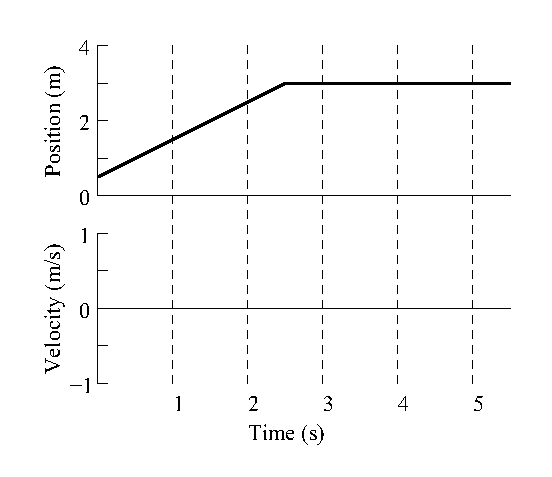
\includegraphics{relating/relating_fig1.eps} \par}
%\vspace{0.3cm}
\begin{lab_groupplot}*{\makegroupverticals[2]{2.5}{0}{5}}
					[lab_grid,
	group style={
		group size=1 by 2,
		xlabels at=edge bottom,
%		xticklabels at=edge bottom,
		vertical sep=0.4in
		},
	width=4in,
	height=2in,
	xlabel=Time (s),
	xmin=0, xmax=5,
	minor x tick num=1,
	]
\nextgroupplot[
	ymin=0,ymax=4, 
	ylabel={Position (m)},
	ylabel_align={-1},
	]
\addplot coordinates{(0,0.5) (2.5,3) (5,3)};

\nextgroupplot[
	ymin=-1,ymax=1, 
	ytick distance = 1, 
	minor y tick num=1, 
	y0_line,
	ylabel={Velocity (m/s)},
	]
\end{lab_groupplot}


(b) After each person in your group has sketched a prediction, test your prediction
by matching the position \textit{vs.}~time graph shown. When you have made a good duplicate
of the position graph, sketch your actual graph over the existing position vs. time graph.
Use a solid line to draw the actual velocity graph on the same graph with
your prediction. (Do not erase your prediction).

(c) How would the position graph be different if you moved faster? Slower? 
\answerspace{15mm}

(d) How would the velocity graph be different if you moved faster? Slower? 
\answerspace{15mm}

\textbf{Activity 2: Average Velocity Calculations} 

(a) Find your average velocity \emph{during the time you were moving at constant speed} from your velocity graph in the previous activity. To do this, use the \textbf{Statistics} function on the graph menu bar to determine the average velocity and the standard deviation on the \emph{left} part of the graph (where the velocity is approximately constant). See \textbf{Appendix \ref{capstone}: Capstone} for instructions on how to do this.

%Velocity values (m/s) \rule{0.5in}{0.1pt} \rule{0.5in}{0.1pt} \rule{0.5in}{0.1pt} \rule{0.5in}{0.1pt} \rule{0.5in}{0.1pt} \rule{0.5in}{0.1pt} \rule{0.5in}{0.1pt} \rule{0.5in}{0.1pt} \rule{0.5in}{0.1pt} \rule{0.5in}{0.1pt}
\answerspace{5mm}

Average value of the velocity: \rule{1.0in}{0.1pt} m/s

Standard deviation: \rule{1.0in}{0.1pt} m/s     (This can be taken as an uncertainty.)

Average velocity with uncertainty: \rule{1.5in}{0.1pt} m/s

(b) Average velocity during a particular time interval can also be calculated
as the change in position divided by the change in time. (The change in position
is often called the displacement.) By definition, this is also the slope of
the position \textit{vs.}~time graph for that time period. Select the position vs. time graph and open the \textbf{Delta Tool} function on the graph menu bar.  Set the cursor on one point on the position graph, right click on this point and select Show Delta Tool.  There will then be two cursors.  Set one cursor on one point on the position graph and the other on another point on the graph.  The changes in position and time will then be shown on the graph. (For a more accurate answer, use two points as far apart
as possible but still typical of the motion, \emph{and within the time 
interval over which you took velocity readings in part (a)}.) 
Record the values of \( \Delta x\) and \( \Delta t\) here:
\answerspace{10mm}

(c) Divide the change in position by the change in time to calculate the average velocity.  Show your calculation here:
\answerspace{15mm}

(d) Is the average velocity positive or negative? Is this what you expected? 
\answerspace{15mm}

\pagebreak[2]
(e) Does the average velocity you just calculated from the position graph fall within the range of values determined in part (a) from the velocity graph? Would you expect them to agree? How would you account for any differences?
\vspace{20mm}

\textbf{Activity 3: Finding Position from a Velocity Graph }

(a) Carefully study the velocity graph that follows. Using a dashed line, sketch your prediction of the corresponding position graph on the top set of axes.
(Assume that you started at the 1-meter mark.)

%\vspace{0.3cm}
%{\par\centering 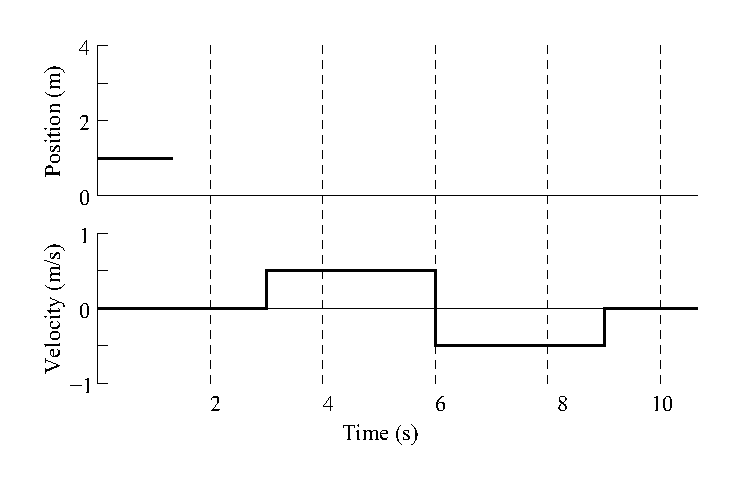
\includegraphics{relating/relating_fig2.eps} \par}
%\answerspace{0.3cm}
\begin{lab_groupplot}*{\makegroupverticals[2]{3,6,9}{0}{11}}
					[lab_grid,
	group style={
		group size=1 by 2,
		xlabels at=edge bottom,
%		xticklabels at=edge bottom,
		vertical sep=0.5in
		},
	width=5in,
	height=2in,
	xlabel=Time (s),
	xmin=0, xmax=11,
	xtick distance = 2,
	minor x tick num=1,
	minor y tick num=1,
	]
\nextgroupplot[
	ymin=0,ymax=4, 
	ytick distance = 2,
	ylabel={Position (m)},
	ylabel_align={-1},
	]
\addplot coordinates{(0,1) (1.5,1)};

\nextgroupplot[
	ymin=-1,ymax=1, 
	ytick distance = 1, 
	minor y tick num=1, 
	ylabel={Velocity (m/s)},
	y0_line,
	]
\addplot coordinates{(0,0) (3,0) (3,0.5) (6,0.5) (6,-0.5) (9,-0.5) (9,0) (11,0)};
\end{lab_groupplot}

(b) After each person has sketched a prediction, do your group's best to duplicate the bottom (velocity \textit{vs.}~time) graph by walking. When you have made a good duplicate of the velocity \textit{vs.}~time graph, draw your actual result over the existing velocity \textit{vs.}~time graph. Use a solid line on the top graph to draw the actual position vs. time graph on the same axes with your prediction. Do not erase your prediction.

(c) How can you tell from a velocity \textit{vs.}~time graph that the moving object has
changed direction?
\answerspace{10mm}

(d) What is the velocity at the moment the direction changes? 
\answerspace{10mm}

(e) Is it possible to actually move your body (or an object) to make vertical
lines on a position \textit{vs.}~time graph? Why or why not? What would the velocity
be for a vertical section of a position \textit{vs.}~time graph? 
\answerspace{10mm}

\pagebreak[2]
(f) How can you tell from a position \textit{vs.}~time graph that your motion is steady
(motion at a constant velocity)? 
\answerspace{10mm}

(g) How can you tell from a velocity \textit{vs.}~time graph that your motion is steady
(constant velocity)? 
\answerspace{20mm}

\textbf{Homework} 

1. Draw the velocity graphs for an object whose motion produced the position-time
graphs shown below on the left.  Note: Unlike most real objects, you can assume these objects can
change velocity so quickly that it looks instantaneous with this time scale.

\begin{center}
\begin{lab_axis}[lab_grid,
	height=1.6in, width=2in,
	xmin=0,xmax=5,
	xlabel={Time (s)},
	ymin=0,ymax=4,
	ylabel={Position (m)},
	xtick distance=1,	 ytick distance=1,
	]
\addplot coordinates{(0,0) (4,4)};
\end{lab_axis}
\hspace{0.3in}
\begin{lab_axis}[lab_grid,
	height=1.6in, width=2in,
	xmin=0,xmax=5,
	xlabel={Time (s)},
	ymin=-2,ymax=2,
	ylabel={Velocity (m/s)},
	xtick distance=1,	 ytick distance=1,
	]
\end{lab_axis}
\end{center}

\begin{center}
\begin{lab_axis}[lab_grid,
	height=1.6in, width=2in,
	xmin=0,xmax=5,
	xlabel={Time (s)},
	ymin=0,ymax=4,
	ylabel={Position (m)},
	xtick distance=1,	 ytick distance=1,
	]
\addplot coordinates{(0,0) (1,2) (5,4)};
\end{lab_axis}
\hspace{0.3in}
\begin{lab_axis}[lab_grid,
	height=1.6in, width=2in,
	xmin=0,xmax=5,
	xlabel={Time (s)},
	ymin=-2,ymax=2,
	ylabel={Velocity (m/s)},
	xtick distance=1,	 ytick distance=1,
	]
\end{lab_axis}
\end{center}

\begin{center}
\begin{lab_axis}[lab_grid,
	height=1.6in, width=2in,
	xmin=0,xmax=5,
	xlabel={Time (s)},
	ymin=0,ymax=4,
	ylabel={Position (m)},
	xtick distance=1,	 ytick distance=1,
	]
\addplot coordinates{(0,0) (2,2) (5,1)};
\end{lab_axis}
\hspace{0.3in}
\begin{lab_axis}[lab_grid,
	height=1.6in, width=2in,
	xmin=0,xmax=5,
	xlabel={Time (s)},
	ymin=-2,ymax=2,
	ylabel={Velocity (m/s)},
	xtick distance=1,	 ytick distance=1,
	]
\end{lab_axis}
\end{center}

%\vspace{0.3cm}
%{\par\centering 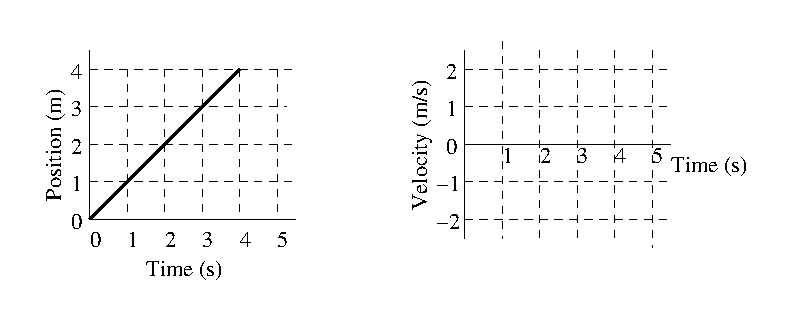
\includegraphics{relating/relating_fig3.eps} \par}
%\vspace{0.3cm}
%
%\vspace{0.3cm}
%{\par\centering 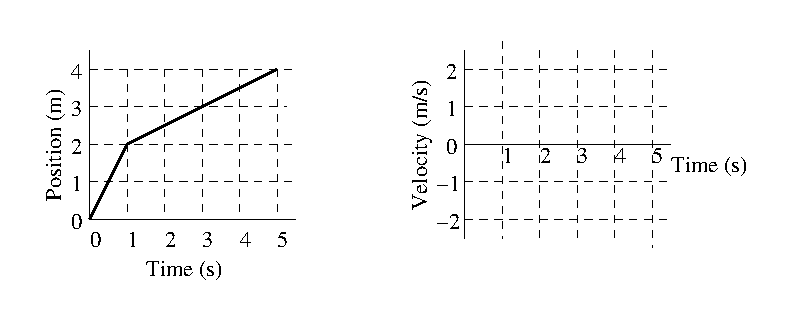
\includegraphics{relating/relating_fig4.eps} \par}
%\vspace{0.3cm}
%
%\vspace{0.3cm}
%{\par\centering 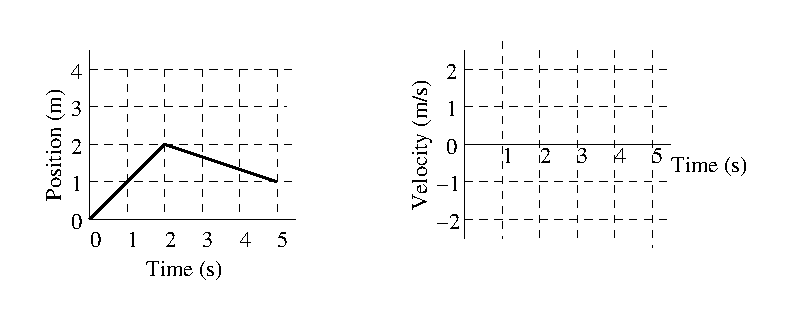
\includegraphics{relating/relating_fig5.eps} \par}
%\vspace{0.3cm}

\pagebreak[3]
2. Draw careful graphs below of position and velocity for a cart that (a) moves
away from the origin at a slow and steady (constant) velocity for the first
5 seconds; (b) moves away at a medium-fast, steady (constant) velocity for the
next 5 seconds; (c) stands still for the next 5 seconds; (d) moves toward the
origin at a slow and steady (constant) velocity for the next 5 seconds; (e)
stands still for the last 5 seconds.

%\vspace{0.3cm}
%{\par\centering 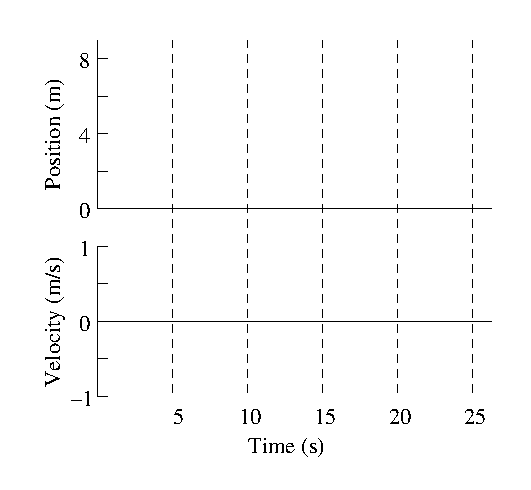
\includegraphics{relating/relating_fig6.eps} \par}
%\vspace{0.3cm}
\begin{lab_groupplot}*{}
					[lab_grid,
	group style={
		group size=1 by 2,
		xlabels at=edge bottom,
%		xticklabels at=edge bottom,
		vertical sep=0.3in,
		},
	width=4in,
	height=2in,
	xlabel=Time (s),
	xmin=0, xmax=25,
	minor x tick num=1
	]
\nextgroupplot[
	ymin=0,ymax=8, 
	ylabel={Position (m)},
	ylabel_align={-1},
	]
\nextgroupplot[
	ymin=-1,ymax=1, 
	ytick distance = 1, 
	minor y tick num=1, 
	y0_line,
	ylabel={Velocity (m/s)},
	]
\end{lab_groupplot}

